% =====================================================================
% Springer Nature (sn-jnl) template conversion
% Paper: Kelvin Mode Suppression in Atomic Orbitals: A Vortex-Filament Gap
% Author: Omar Iskandarani
% Date (source): 2025-12-14
% Affiliation: Independent Researcher, Groningen, The Netherlands
% License: © 2025 Omar Iskandarani. All rights reserved.
% DOI: 10.5281/zenodo.18018084
% =====================================================================

% =========================
% 1) Document class choice
% =========================
% \documentclass[referee,pdflatex,sn-mathphys-num]{sn-jnl} % double-spacing option for review
\documentclass[pdflatex,sn-mathphys-num]{sn-jnl}

% =========================
% 2) Core packages (lean)
% =========================
\usepackage[T1]{fontenc}
\usepackage[utf8]{inputenc}
\usepackage{lmodern}
\usepackage{microtype}
\usepackage{graphicx}
\usepackage{booktabs}
\usepackage{amsmath,amssymb,amsfonts}
\usepackage{bm}
\usepackage{siunitx}
% \usepackage{physics}

% TikZ/PGFPlots (used by your figures)
\usepackage{tikz}
\usepackage{pgfplots}
\usepackage{pgfplotstable}
\usepackage{caption}
\pgfplotsset{compat=newest}

% ====================================
% 3) Paper metadata macros (edit here)
% ====================================
\newcommand{\papertitle}{Spectroscopic Constraints on Kelvin-Like Internal Modes\\ in Effective Filament Models of Atomic Bound States}
\newcommand{\papershorttitle}{Kelvin-Like Internal Modes in Atomic Bound States}
\newcommand{\paperdoi}{10.5281/zenodo.18018084}
\newcommand{\paperorcid}{0009-0006-1686-3961}
\newcommand{\paperemail}{info@omariskandarani.com}
\newcommand{\papercity}{Groningen}
\newcommand{\papercountry}{The Netherlands}
\newcommand{\paperkeywords}{Kelvin modes, effective filament models, atomic spectroscopy, excitation gap, low-energy reduction}

\raggedbottom

\begin{document}

% =========================
% 5) Title + author block
% =========================
    \title[\papershorttitle]{\papertitle}

    \author*[1]{\fnm{Omar} \sur{Iskandarani}}\email{\paperemail}
    \affil*[1]{\orgname{Independent Researcher}, \orgaddress{\city{\papercity}, \country{\papercountry}}}

% =========================
% 6) Abstract + keywords
% =========================
    \abstract{%
        We analyze a class of effective bound-state models in which an atomic electron is supplemented by an internal helical excitation sector with Kelvin-like dispersion. The central question is whether such internal modes can remain compatible with precision atomic spectroscopy. We derive a conditional decoupling bound: if the internal sector couples to an observed orbital level with efficiency $\lambda_n$ and is populated at an effective scale $T_{\mathrm{eff}}$, then a spectral gap $\Delta_K$ suppresses the induced level shift by a Boltzmann factor, whereas an ungapped sector lacks any generic exponential protection. The resulting spectroscopic constraint is parametric, not absolute: it bounds the allowed region in $(\lambda_n,N_K,T_{\mathrm{eff}},\Delta_K)$ space rather than predicting a unique value of $\Delta_K$. A separate dispersion-based estimate places the onset of the lowest internal mode in the $\mathcal{O}(10^2\,\mathrm{eV})$ range for fiducial filament parameters, with shorter effective loop lengths pushing the scale upward. Taken together, the spectroscopic bound and the onset estimate define a consistency window, rather than a sharp prediction, for any atomic bound-state model endowed with an internal filamentary or Kelvin-like excitation sector.%
    }

    \keywords{\paperkeywords}

    \maketitle

% Global dimensionless temperature ratio
    \newcommand{\epsilonK}{\varepsilon_K} % Dimensionless temperature ratio

% ============================================================
    \section{Introduction}\label{sec:intro}
        Hydrodynamic and vortex-based models of matter trace back to Kelvin and Helmholtz \cite{Helmholtz1858,Kelvin1867}. Modern superfluid dynamics and quantum turbulence have renewed interest in vortex filaments as fundamental excitations \cite{Onsager1949,Feynman1955,Barenghi2014}.

        In that broader context, it is natural to ask whether an atomic bound state might admit an \emph{effective} description in which the usual orbital degree of freedom is accompanied by an internal filament-like excitation sector.

        This paper does not attempt to establish such a microscopic picture as fundamental. Its purpose is narrower: to derive a consistency condition. If an internal Kelvin-like sector exists and couples to bound electronic states, then atomic spectroscopy immediately constrains its low-energy behavior. The question is therefore not whether one prefers a filament interpretation, but whether any such internal sector can remain invisible at atomic energies.

        The main result is simple. An ungapped Kelvin-like spectrum generically leads to thermodynamic or kinematic corrections that are too large to be compatible with hydrogenic line stability. A gapped spectrum avoids this problem: below the gap, the internal sector is effectively frozen and the reduced low-energy dynamics are described by the usual stationary Schr\"odinger equation. In that sense, the paper should be read as a no-go / decoupling result for internal-mode completions of atomic bound states.

% ============================================================
    \section{Kelvin Waves on Vortex Filaments}\label{sec:kelvin}
        For a thin filament with circulation $\Gamma$ and core radius $\xi$, small-amplitude Kelvin waves satisfy \cite{LordKelvin1880,Barenghi2014}
        \begin{equation}
            \omega(k) \simeq \frac{\Gamma}{4\pi} k^2
            \left[
                \ln\!\left(\frac{1}{|k|\xi}\right) + C_0
            \right],
            \label{eq:kelvin_dispersion}
        \end{equation}
        with $C_0=\mathcal{O}(1)$. For a closed filament of length $L$,
        \begin{equation}
            k_m = \frac{2\pi m}{L}, \quad m=1,2,\dots,\qquad
            \omega_m \propto \frac{\Gamma m^2}{L^2}.
        \end{equation}
        For hydrogenic orbitals $r_n=a_0 n^2$, implying $L_n\sim 2\pi a_0 n^2$, Kelvin frequencies soften rapidly with principal quantum number $n$.

% ============================================================
    \section{Thermodynamic Constraint from Atomic Spectroscopy}\label{sec:constraint}
        Suppose an atomic bound state carries, in addition to its orbital energy $E_n^{(0)}$, an internal contribution from Kelvin-like modes,
        \begin{equation}
            E_n^{\mathrm{eff}}(T_{\mathrm{eff}})
            =
            E_n^{(0)} + \delta E_n(T_{\mathrm{eff}}),
        \end{equation}
        where $T_{\mathrm{eff}}$ is not necessarily a literal thermodynamic temperature, but an effective population scale for the internal sector.

        If the internal modes are ungapped, then the low-energy correction generically admits a polynomial expansion,
        \begin{equation}
            \delta E_n(T_{\mathrm{eff}})
            =
            - a_n T_{\mathrm{eff}}^2 + \mathcal{O}(T_{\mathrm{eff}}^4),
            \label{eq:poly_correction}
        \end{equation}
        or an analogous low-order dependence determined by the density of states. Precision spectroscopy severely limits such terms. The point of the present argument is not the exact coefficient in this expansion, but the scaling: any low-energy polynomial sensitivity of the orbital sector to internal Kelvin-like modes is strongly constrained.

        Thus, absent additional structure, an ungapped internal sector is generically incompatible with the observed sharpness and stability of hydrogenic energy levels.

% ============================================================
    \section{Gapped Kelvin Spectrum}\label{sec:gap}
        The minimal decoupling mechanism is an excitation gap $\Delta_K$ in the internal spectrum: the first excitation costs $\Delta_K$, and higher modes obey $E_{m,n}\ge\Delta_K$. A convenient Hamiltonian is
        \begin{equation}
            H_K^{(n)} = \sum_m \left[
                                   (\Delta_K+\delta E_{m,n})\, b_{mn}^\dagger b_{mn}
                                   + \frac{1}{2}(\Delta_K+\delta E_{m,n})
            \right].
        \end{equation}
        The microscopic origin of $\Delta_K$ is left open here; in an effective filament picture it may arise from topology, curvature, torsion, core structure, or geometric constraints on admissible excitations \cite{Ricca1996}.

        A dimensional estimate supports the required magnitude of $\Delta_K$. For a filament with circulation $\Gamma$ and core radius $\xi$, the tension $T_f \sim \rho \, \Gamma^2/(4\pi \xi^2)$ sets a characteristic bending energy for the first Kelvin mode. Taking the mode wavelength to be of order the loop length $L$, one obtains $\Delta_K \sim \Gamma^2/(4\pi \xi L)$ up to logarithmic corrections. With $\Gamma = h/m_e$, $\xi \sim 10^{-15}\,\mathrm{m}$, and $L \sim 10^{-10}\,\mathrm{m}$, this gives $\Delta_K = \mathcal{O}(10^2\text{--}10^3\,\mathrm{eV})$, consistent with the phenomenological scale used below.

% ============================================================
    \section{Low-Temperature Thermodynamics}\label{sec:lowT}
        The dimensionless temperature ratio
        \[
            \epsilonK = \frac{k_B T}{\Delta_K} \ll 1
        \]
        characterizes the low-temperature (Kelvin-frozen) regime.
        For a single gapped bosonic mode \cite{Pathria2011},
        \begin{equation}
            Z = \frac{1}{1 - e^{-\beta\Delta_K}}, \qquad
            U = \frac{\Delta_K}{e^{\beta\Delta_K} - 1}, \qquad
            \beta = (k_B T)^{-1}.
        \end{equation}
        In the limit $\epsilonK \ll 1$,
        \begin{equation}
            U \simeq \Delta_K e^{-1/\epsilonK},
        \end{equation}
        so entropy and heat capacity are exponentially suppressed.

        \begin{figure}[htbp]
            \centering
            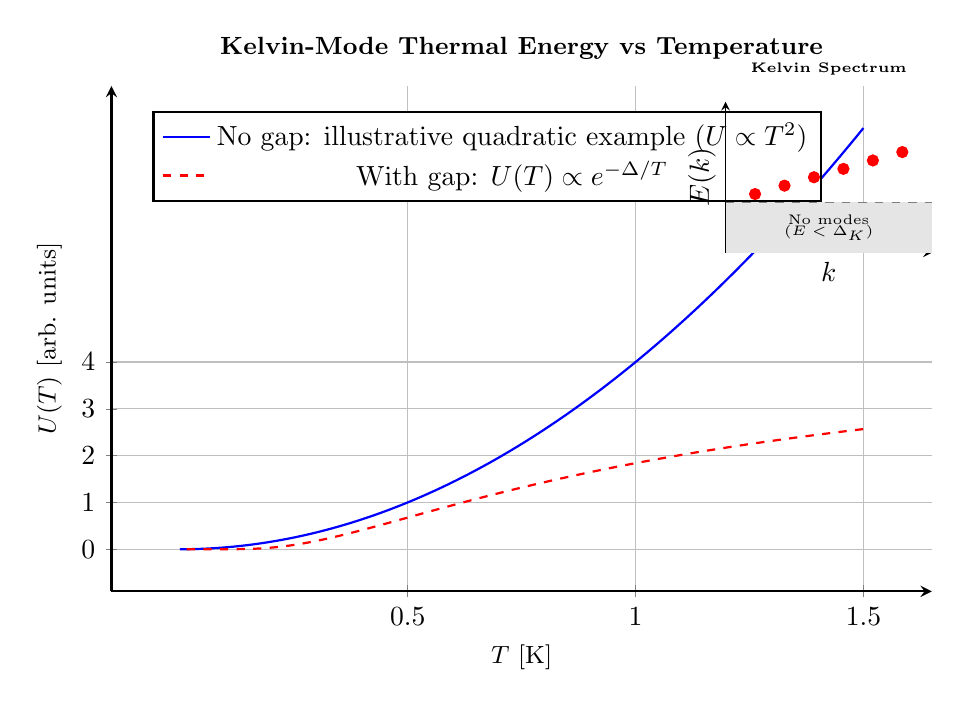
\begin{tikzpicture}
% MAIN PLOT: Thermal Energy vs Temperature
                \begin{axis}[
                width=12cm,
                height=8cm,
                xlabel={$T$ [K]},
                ylabel={$U(T)$ [arb. units]},
                legend style={at={(0.05,0.95)}, anchor=north west},
                domain=0:1.5,
                samples=100,
                axis lines=left,
                enlargelimits=true,
                grid=both,
                xtick={0.5,1.0,1.5},
                ytick={0,1,2,3,4},
                xlabel style={font=\small},
                ylabel style={font=\small},
                title={Kelvin-Mode Thermal Energy vs Temperature},
                title style={font=\bfseries\small},
                thick
                ]
% No Gap: U ~ T^2
                \addplot[blue,thick] {4*x^2};
                \addlegendentry{No gap: illustrative quadratic example ($U \propto T^2$)}
% With Gap: U ~ exp(-Δ/T)
                \addplot[red,thick,dashed] {5*exp(-1/x)};
                \addlegendentry{With gap: $U(T) \propto e^{-\Delta/T}$}
                \end{axis}

% INSET: Energy spectrum with gap
                \begin{scope}[shift={(7.8,4.3)}]
                    \begin{axis}[
                    width=4.2cm,
                    height=3.5cm,
                    title={Kelvin Spectrum},
                    title style={font=\bfseries\tiny},
                    xlabel={$k$},
                    ylabel={$E(k)$},
                    axis lines=left,
                    ticks=none,
                    xmin=0, xmax=3.5,
                    ymin=0, ymax=4.5,
                    xtick=\empty,
                    ytick=\empty,
                    clip=false
                    ]
                    \fill[gray!20] (axis cs:0,0) rectangle (axis cs:3.5,1.5);
                    \draw[dashed, gray] (axis cs:0,1.5) -- (axis cs:3.5,1.5);
                    \foreach \x in {0.5,1.0,1.5,2.0,2.5,3.0} {
                        \addplot[only marks, mark=*, red] coordinates {(\x, {1.5 + 0.5*\x})};
                    }
                    \node[align=center,font=\tiny] at (axis cs:1.75,0.75) {No modes\\[-0.3em]($E<\Delta_K$)};
                    \end{axis}
                \end{scope}
            \end{tikzpicture}
            \caption{Schematic comparison of internal-mode thermal energy with and without an excitation gap $\Delta_K$. The ungapped curve is shown here as one illustrative quadratic example only; the manuscript does not assume a universal $T^2$ law. The point is the contrast between algebraic growth and Boltzmann suppression. Inset: discrete spectrum with a forbidden band $E<\Delta_K$.}
            \label{fig:kelvin-gap}
        \end{figure}

        \begin{figure}[htbp]
            \centering
            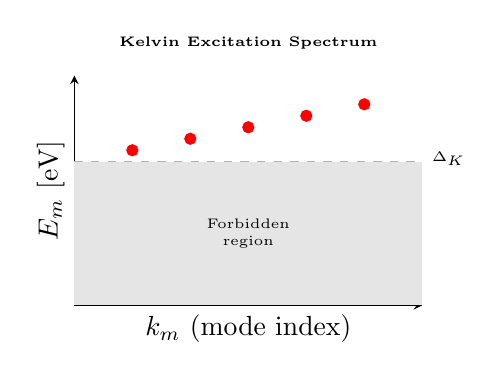
\begin{tikzpicture}
                \begin{axis}[
                width=6cm,
                height=4.5cm,
                title={Kelvin Excitation Spectrum},
                title style={font=\bfseries\tiny},
                xlabel={$k_m$ (mode index)},
                ylabel={$E_m$ [eV]},
                axis lines=left,
                ticks=none,
                xmin=0, xmax=6,
                ymin=0, ymax=800,
                clip=false
                ]
                \pgfmathsetmacro{\DeltaK}{500} % eV gap
                \fill[gray!20] (axis cs:0,0) rectangle (axis cs:6,\DeltaK);
                \draw[dashed, gray!60] (axis cs:0,\DeltaK) -- (axis cs:6,\DeltaK);
                \node[align=center,font=\tiny] at (axis cs:3,250) {Forbidden\\ region};
                \foreach \x in {1,2,3,4,5} {
                    \addplot[only marks, mark=*, red, mark size=2pt] coordinates {(\x, {\DeltaK + 40*\x})};
                }
                \node[anchor=west,font=\tiny] at (axis cs:6,\DeltaK+10) {$\Delta_K$};
                \end{axis}
            \end{tikzpicture}
            \caption{Illustrative Kelvin excitation spectrum with a gap $\Delta_K=\SI{500}{\electronvolt}$. Shaded band: $E<\Delta_K$.}
            \label{fig:kelvin-thermal-suppression}
        \end{figure}

        For finitely many Kelvin modes,
        \begin{equation}
            U_K^{(n)}(T) \lesssim N_K \Delta_K \exp\!\left(-\frac{\Delta_K}{k_B T}\right),
        \end{equation}
        replacing the dangerous polynomial scaling of the ungapped case.

        \begin{didactic}
            \emph{Takeaway.} With a gap, thermal activation is exponentially small: $U\sim e^{-\Delta_K/k_BT}$, not $\sim T^2$.
        \end{didactic}

% ============================================================
    \section{Required Gap Scale}\label{sec:required_gap}
        Let $\delta E_{\mathrm{spec}}$ denote the maximum spectroscopy-compatible correction to a low-lying level, and let $\lambda_n$ denote the efficiency with which the internal sector couples to shifts of orbital level $n$. The abstract's parameter tuple $(\lambda_n,N_K,T_{\mathrm{eff}},\Delta_K)$ is related to the compact phenomenological bound below by absorbing $\lambda_n$ into the effective scale of the numerator (equivalently, one may regard $N_K$ as an effective mode count already weighted by coupling). Then a sufficient condition for decoupling is
        \begin{equation}
            N_K \Delta_K
            \exp\!\left(-\frac{\Delta_K}{k_B T_{\mathrm{eff}}}\right)
            \lesssim
            \delta E_{\mathrm{spec}}.
            \label{eq:general_bound}
        \end{equation}
        Equivalently,
        \begin{equation}
            \frac{\Delta_K}{k_B T_{\mathrm{eff}}}
            \gtrsim
            \ln\!\left(\frac{N_K \Delta_K}{\delta E_{\mathrm{spec}}}\right).
            \label{eq:log_bound}
        \end{equation}
        Nevertheless, the dependence is only logarithmic in $N_K \Delta_K/\delta E_{\mathrm{spec}}$. The numerical non-triviality of Eq.~\eqref{eq:log_bound} therefore depends on the assumed effective occupation scale: for room-temperature populations the bound may require only an eV-scale gap, whereas substantially larger $T_{\mathrm{eff}}$ pushes the required gap above ordinary atomic binding energies. The present paper does not independently derive a specific range for $T_{\mathrm{eff}}$; accordingly, Eq.~\eqref{eq:log_bound} should be read as a conditional constraint on parameter space rather than as an absolute numerical prediction. Appendix~\ref{app:first_kelvin} then supplies an independent fiducial onset estimate for the lowest internal mode. Taken together, the spectroscopic bound and the dispersion estimate define a consistency window rather than a sharp prediction.

        For spectroscopically small $\delta E_{\mathrm{spec}}$, the right-hand side is typically a number of order a few tens. As one illustrative scenario, if the effective internal-sector population scale lies in the range
        \begin{equation}
            T_{\mathrm{eff}} \sim 10^4\text{--}10^5\,\mathrm{K},
        \end{equation}
        then the required gap naturally falls in the range
        \begin{equation}
            \Delta_K \sim 10^2\text{--}10^3\,\mathrm{eV}.
        \end{equation}
        This is parametrically above ordinary atomic binding energies and therefore sufficient, in that regime, to keep the internal Kelvin-like sector inactive in standard atomic spectroscopy.

% ============================================================
    \section{Reduced Low-Energy Description}\label{sec:schrodinger}
        \begin{figure}[ht]
            \centering
            
\includegraphics[width=0.85\textwidth]{hydro_energy_levels}
            \caption{\textbf{Schematic low-energy level structure} for $n = 1,2,3,4$. The displayed scaling is intended only as a phenomenological illustration of hydrogenic behavior in the reduced theory after the internal Kelvin-like sector is frozen out.}
            \label{fig:hydrodynamic_levels}
        \end{figure}

        Once the internal sector is frozen, the remaining low-energy orbital dynamics are described by the standard single-particle effective Hamiltonian,
        \begin{equation}
            H_{\mathrm{eff}}
            =
            -\frac{\hbar^2}{2m_e}\nabla^2 + V_{\mathrm{eff}}(r),
        \end{equation}
        \begin{equation}
            -\frac{\hbar^2}{2m_e}\nabla^2\psi + V_{\mathrm{eff}}(r)\psi = E\psi.
        \end{equation}
        In the present paper, this is not claimed as a derivation of quantum mechanics from hydrodynamics. Rather, it is the reduced low-energy description that remains after the internal Kelvin-like sector has been shown to decouple exponentially.

% ============================================================
    \section{Failure of Ungapped Internal Modes}\label{sec:catastrophe}
        If Kelvin modes couple thermodynamically to orbitals, one can parameterize
        \begin{equation}
            U_{\mathrm{Kelvin},n}(T_\ast)
            =
            a_n T_\ast^2 + \mathcal{O}(T_\ast^4),
            \qquad
            E_n^{\mathrm{eff}} = E_n^{(0)} - a_n T_\ast^2.
        \end{equation}
        A naive elastic estimate gives
        \begin{equation}
            a_n^{\text{naive}} \sim 10^{-39}\,\mathrm{J/K^2},
        \end{equation}
        while spectroscopy requires
        \begin{equation}
            a_n \lesssim 10^{-62}\,\mathrm{J/K^2}.
        \end{equation}
        The gap is therefore essential: without it, the $1/n^2$ spectrum collapses.

% ============================================================
    \section{Discussion and Outlook}\label{sec:outlook}
        The result of this paper is a conditional consistency bound. Any effective atomic bound-state model endowed with an internal Kelvin-like filament sector faces a sharp spectroscopic requirement: once the parameters $(N_K,T_{\mathrm{eff}},\Delta_K)$ and the spectroscopic tolerance $\delta E_{\mathrm{spec}}$ are specified, Eq.~\eqref{eq:log_bound} determines whether the internal sector is safely decoupled from observed low-energy lines. Qualitatively, if that sector is ungapped, low-energy corrections are generically too large; if it is gapped, the correction is exponentially suppressed and ordinary atomic quantum mechanics is recovered as the reduced low-energy theory.

        The main consequence is qualitative but robust. A nonzero gap provides exponential protection. An ungapped sector can still be compatible with spectroscopy, but only if some additional mechanism suppresses either the low-energy density of states, the effective occupation, or the coupling to observed level shifts. The non-triviality of the bound likewise depends on how strongly the internal sector couples to those shifts: if the effective coupling were itself extremely small, the constraint would become correspondingly weak. In that sense, the present argument is most informative in regimes where the internal sector is populated at a non-negligible effective scale and where the transfer of internal excitation energy into observable level shifts is not itself exponentially suppressed. Determining that coupling from a specific microscopic mechanism is beyond the scope of the present phenomenological note, but that mechanism would set how restrictive Eq.~\eqref{eq:log_bound} becomes in practice.

        This framing yields a narrow and testable claim. The relevant experimental question is not whether atomic structure is ``really'' filamentary, but whether any additional internal sector activates above a threshold in the approximate range
        \begin{equation}
            \Delta_K \sim 10^2\text{--}10^3\,\mathrm{eV}.
        \end{equation}
        Potential signatures would then appear not in ordinary spectroscopy, where the sector is frozen, but in threshold-like inelastic channels, anomalous broadening, or additional loss mechanisms once the excitation scale is crossed.

        The paper therefore motivates a focused search strategy: high-field or high-energy probes of bound electrons, rather than reinterpretation of standard low-energy spectroscopy. At low energy the internal sector must be silent; at sufficiently high excitation, it may become observable.

% ============================================================
        \appendix
    \section*{Appendix A: Estimate of First Kelvin Mode Energy}\label{app:first_kelvin}
        For the first mode ($m=1$) in the ground state ($n=1$), take
        \begin{equation}
            L = 2\pi a_0 \approx \SI{3.3249e-10}{m},
            \qquad
            \Gamma = \frac{h}{m_e} \approx \SI{7.2739e-4}{m^2/s},
        \end{equation}
        \begin{equation}
            k_1 = \frac{2\pi}{L} \approx \SI{1.8897e10}{m^{-1}}.
        \end{equation}
        Using $\xi = \SI{1e-15}{m}$ gives
        \begin{equation}
            k_1\xi \approx 1.8897\times 10^{-5},
            \qquad
            \ln\!\left(\frac{1}{k_1\xi}\right)\approx 10.876.
        \end{equation}
        With $C_0=1$, Eq.~\eqref{eq:kelvin_dispersion} yields
        \begin{equation}
            \omega_1 \simeq \frac{\Gamma}{4\pi} k_1^2 \!\left[ \ln\!\left( \frac{1}{k_1 \xi} \right) + 1 \right]
            \approx \SI{2.45e17}{rad/s},
        \end{equation}
        and therefore
        \begin{equation}
            E_1=\hbar\omega_1 \approx \SI{1.62e2}{eV}.
        \end{equation}
        Since $E_1\propto L^{-2}$ up to logarithmic corrections, modest geometric shortening of the effective loop readily lifts the onset into the sub-keV or keV regime.

        For the illustrative parameter sweep reported above, the onset window may be summarized as
        \begin{equation}
            \SI{1e2}{\electronvolt} \lesssim E_1 \lesssim \SI{1.3}{\kilo\electronvolt},
        \end{equation}
        where the lower end corresponds to Bohr-scale loop length with softer regularization and the upper end to a modestly shortened effective loop with the same fiducial circulation scale. The dispersion estimate therefore supplies a fiducial onset scale and a geometry-dependent window, not a unique prediction. This is exactly the role it plays in the main text, where it is combined with the conditional spectroscopic bound to identify a consistency region for viable internal-mode models. Geometry-dependent corrections or additional curvature contributions can shift the threshold by a factor of a few, but the fiducial scale is already well above ordinary atomic binding energies.

% ============================================================
% Back matter (Springer Nature)
% ============================================================
        \backmatter
        \bmhead{Declarations}

        \subsection*{Funding}
            Not applicable.

        \subsection*{Competing interests}
            The author declares no competing interests.

        \subsection*{Ethics approval}
            Not applicable.

        \subsection*{Consent to participate}
            Not applicable.

        \subsection*{Consent for publication}
            Not applicable.

        \subsection*{Data availability}
            Not applicable.

        \subsection*{Materials availability}
            Not applicable.

        \subsection*{Code availability}
            Not applicable.

        \subsection*{Author contributions}
            O.I. conceived the study, developed the analysis, performed the derivations, and wrote the manuscript.

% ============================================================
% References
% ============================================================
            \begin{thebibliography}{99}

                \bibitem{Helmholtz1858}
                H.~Helmholtz,
                ``On Integrals of the Hydrodynamical Equations Which Express Vortex Motion,''
                \emph{J. Reine Angew. Math.} \textbf{55}, 25--55 (1858).

                \bibitem{Kelvin1867}
                W.~Thomson (Lord Kelvin),
                ``On Vortex Atoms,''
                \emph{Proc. R. Soc. Edinburgh} \textbf{6}, 94--105 (1867).

                \bibitem{Onsager1949}
                L.~Onsager,
                ``Statistical Hydrodynamics,''
                \emph{Nuovo Cimento Suppl.} \textbf{6}, 279--287 (1949).

                \bibitem{Feynman1955}
                R.~P.~Feynman,
                ``Application of Quantum Mechanics to Liquid Helium,''
                in \emph{Progress in Low Temperature Physics}, Vol.~1,
                North-Holland (1955).

                \bibitem{LordKelvin1880}
                W.~Thomson (Lord Kelvin),
                ``Vibrations of a Columnar Vortex,''
                \emph{Philosophical Magazine} \textbf{10}, 155--168 (1880).

                \bibitem{Barenghi2014}
                C.~F.~Barenghi, L.~Skrbek, and K.~R.~Sreenivasan,
                ``Introduction to Quantum Turbulence,''
                \emph{Proc. Natl. Acad. Sci. USA} \textbf{111}, 4647--4652 (2014).

                \bibitem{Ricca1996}
                R.~L.~Ricca,
                ``The Contributions of Da Rios and Levi-Civita to Asymptotic Potential Theory and Vortex Filament Dynamics,''
                \emph{Fluid Dynamics Research} \textbf{18}, 245--268 (1996).

                \bibitem{Pathria2011}
                R.~K.~Pathria and P.~D.~Beale,
                \emph{Statistical Mechanics}, 3rd ed.,
                Elsevier (2011).

                \bibitem{AbeOkuyama2011}
                S.~Abe and S.~Okuyama,
                ``Similarity between Quantum Mechanics and Thermodynamics,''
                \emph{Phys. Rev. E} \textbf{83}, 021121 (2011).

                \bibitem{Unruh1976}
                W.~G.~Unruh,
                ``Notes on Black-Hole Evaporation,''
                \emph{Phys. Rev. D} \textbf{14}, 870--892 (1976).

                \bibitem{Madelung1926}
                E.~Madelung,
                ``Quantentheorie in hydrodynamischer Form,''
                \emph{Z. Phys.} \textbf{40}, 322--326 (1926).

                \bibitem{Bohm1952}
                D.~Bohm,
                ``A Suggested Interpretation of the Quantum Theory in Terms of `Hidden' Variables. I.,''
                \emph{Phys. Rev.} \textbf{85}, 166--179 (1952).

                \bibitem{Couder2006}
                Y.~Couder, S.~Proti\`ere, E.~Fort, and A.~Boudaoud,
                ``Dynamical phenomena: Walking and orbiting droplets,''
                \emph{Nature} \textbf{437}, 208 (2005).

                \bibitem{PageWootters1983}
                D.~N.~Page and W.~K.~Wootters,
                \textit{Evolution without evolution: Dynamics described by stationary observables},
                Physical Review D \textbf{27} (1983) 2885.
                doi:10.1103/PhysRevD.27.2885

                \bibitem{Wootters1984}
                W.~K.~Wootters,
                \textit{``Time'' replaced by quantum correlations},
                International Journal of Theoretical Physics \textbf{23} (1984) 701--711.
                doi:10.1007/BF02214098

                \bibitem{SmithAhmadi2020}
                A.~R.~H.~Smith and M.~Ahmadi,
                \textit{Quantum clocks observe classical and quantum time dilation},
                Nature Communications \textbf{11} (2020) 5360.
                doi:10.1038/s41467-020-18264-4

                \bibitem{CastroRuiz2017}
                E.~Castro-Ruiz, F.~Giacomini, and \v{C}.~Brukner,
                \textit{Entanglement of quantum clocks through gravity},
                Proceedings of the National Academy of Sciences \textbf{114} (2017) E2303--E2309.
                doi:10.1073/pnas.1616427114

            \end{thebibliography}

\end{document}